% !TeX root = skript.tex
Das Forschungsfeld der Zufallsgraphen nahm mit den Arbeiten von Gilbert~\cite{gilbert_1959}, sowie Erd\H{o}s und R\'enyi~\cite{erdos_renyi_1960} Anfang der 1960er Jahre an Fahrt auf.
Die beiden Arbeiten definieren Zufallsgraphmodelle, die zunächst für abstrakte Untersuchungen (z.B. die Probabilistische Methode) verwendet wurden.
Bis heute spielen die Modelle in der Netzwerkforschung jeodch eine wichtige Rolle.
Wir werden sie daher bald genauer betrachten, fangen jedoch mit einem einfacheren Modell an.

\section{Der Zufallsgraph $G(n)$}
Ein Zufallsgraph $(\mathbb G, P)$ ist eine Wahrscheinlichkeitsverteilung $P\colon \mathbb G \to [0, 1]$ über einer Menge von Graphen $\mathbb G$.
Oftmals wird der Grundraum $\mathbb G$ durch eine Parameterisierung eingeschränkt; auch $P$ kann parametrisiert sein.

Das \aside{$G(n)$ Graphen} einfachste Modell ist $G(n)$, welches die Gleichverteilung über alle Graphen mit $n$ Knoten beschreibt.
Hierbei ist zu beachten, dass wir mit \emph{alle Graphen} in der Regel entweder alle \emph{gerichteten} oder alle \emph{ungerichteten} Graphen meinen.
Die Details der Analysen in den folgenden Kapiteln hängen von dieser Entscheidung ab --- allerdings ergeben sich meist keine qualitativen Unterschiede.
Daher werden wir oft den für uns einfacheren Fall wählen.
Je nach Wahl, ist der Grundraum von $G(n)$
\begin{eqnarray}
    \mathbb G_\text{ger}(n) &=&
    \twoset{G(V,E)}{|V| = n \land E \subseteq V \times V}\\
    \mathbb G_\text{unge}(n) &=&
    \twoset{G(V,E)}{|V| = n \land  E \subseteq \twoset{\set{u,v}}{u,v \in V \text{ mit } u \ne v}}.
\end{eqnarray}

\noindent Die Wahrscheinlichkeitsverteilung $P$ folgt dann als $P_{\mathbb G(n)}(G) = 1 / | \mathbb G(n) |$, oder konkret:
\begin{eqnarray}
    P_{\mathbb G_\text{ger}(n)}(G) &=& \frac{1}{| \mathbb G_\text{ger}(n) |} = \frac{1}{n^2}\\
    P_{\mathbb G_\text{unge}(n)}(G) &=& \frac{1}{| \mathbb G_\text{unge}(n) |} = \frac{1}{\binom n 2} = \frac{2}{n(n-1)}.
\end{eqnarray}

\begin{figure}[t]
    \begin{center}
        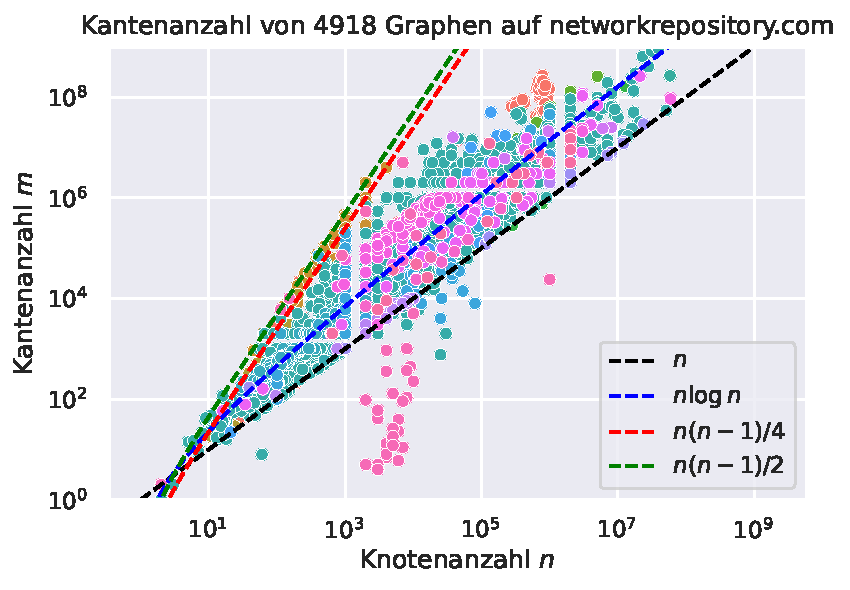
\includegraphics[width=0.5\textwidth]{data/network-rep-edges.pdf}%
        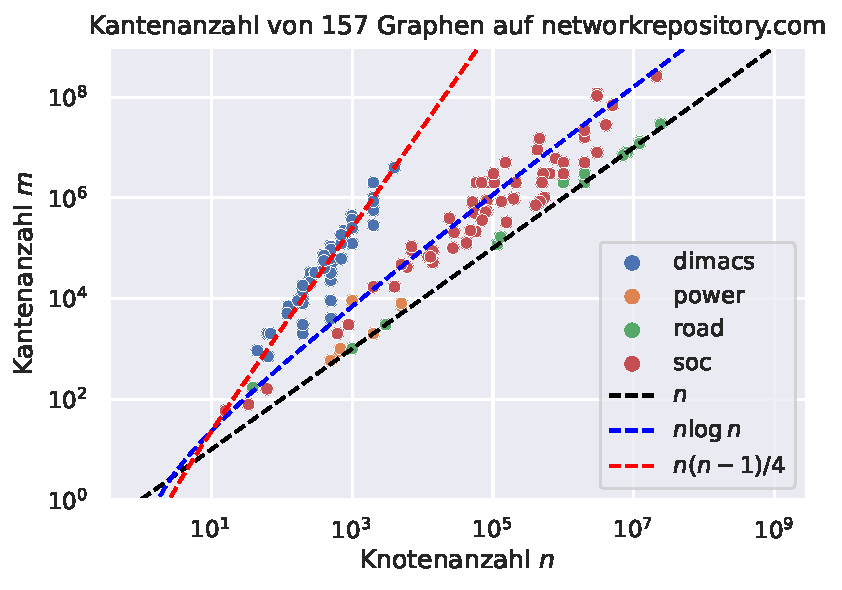
\includegraphics[width=0.5\textwidth]{data/network-rep-edges-thin.pdf}%
    \end{center}
    \caption{
        Die Verteilung der Kantenanzahl in verschiedenen Netzwerken auf~\cite{networkrepository}.
        Die Farben der einzelnen Punkte geben an, aus welchem Bereich die Netzwerke stammen.
    }
    \label{fig:kantenanzahl}
\end{figure}

Ist das $G(n)$ Modell realistisch?
Das hängt davon ab, was wir mit ihm bezwecken und was wir mit \emph{realistisch} meinen.
Es ist aber sicherlich nicht geeignet, um gängige Netzwerke zu beschreiben.
Dies liegt unter anderem daran, dass $G(n)$ oft Graphen mit vielen Kanten erzeugt;
intutitiv hat \glqq jeder zweite Graph\grqq{} mindestens die Hälfte aller möglichen Kanten.

\begin{observation}
    Sei $G(V,E)$ ein Graph, der zufällig aus $G(n)$ mit $n > 1$ gezogen wurde.
    Dann gilt für gerichtete Graphen $\prob{|E| \ge n^2 / 2} \ge 1/2$ und für ungerichtete Graphen $\prob{|E| \ge \binom{n}{2} / 2} \ge 1/2$.
\end{observation}

\begin{proof}
    Im Folgenden betrachen wir nur gerichtete Graphen; der Beweis läuft analog für ungerichtete Graphen.
    Stellen wir uns einen beliebigen Graphen~$G(V, E)$ vor.
    Dann sei $\bar G(V, \bar E)$ sein Komplement, d.h. für alle möglichen Kanten~$e$ gilt: $e \in \bar E \Leftrightarrow e \notin E$.
    Beobachte, dass es eine Bijektion zwischen allen Graphen in $\mathbb G$ und ihren Komplementen gibt: jeder Graph hat ein eineindeutiges Komplement.
    Per Konstruktion gilt außerdem:
    \begin{eqnarray}
        E \cup \bar E &=& V \times V\\
        \Rightarrow |E| + |\bar E| &\ge& n^2\\
        \Rightarrow \max(|E|, |\bar E|) &\ge& n^2 / 2.
    \end{eqnarray}

    Für jeden Graph~$G$ gilt also, dass entweder $G$ selbst oder sein Komplement~$\bar G$ mindestens $n^2 / 2$ Kanten hat.
    Da wir $G$ und $\bar G$ ja mit gleicher Wahrscheinlichkeit ziehen, gilt $\prob{|E| \ge n^2 / 2} \ge 1/2$.
\end{proof}

\section{Kantenanzahl in beobachteten Netzwerken}
Wie viele Kanten haben echte Netzwerke? Hierzu führen wir ein Experiment durch:
wir nutzen die Datenbank \url{https://networkrepository.com/}, die über 5000 Netzwerke aus unterschiedlichen Bereichen enthält~\cite{networkrepository}.
In \cref{fig:kantenanzahl} zeichnen wir die Kantenanzahl als Funktion der Knotenanzahl.
Zwei Eigenschaften fallen direkt auf:
\begin{enumerate}
    \item Die Kantendichte hängt vom Netzwerktyp ab.
    \item Es sind fast immer deutlich weniger als die Hälfte der Kanten vorhanden.
\end{enumerate}

\subsection{Netzwerktypen haben unterschiedliche Kantendichten}
Betrachten wir die erste Beobachtung genauer, indem wir Straßennetze und Freundschaftsnetze vergleichen.
Wir modellieren ein Straßennetz dadurch, dass Adressen (Häuser, Kreuzung, usw.) als Knoten und Straßen als Kanten dargestellt werden.
Diese Netze \aside{Straßennetze} sind im wesentlichen ein zwei-dimensionales Konstrukt.
Wenn wir Tunnel, Brücken und der gleichen ignorieren, verlaufen Straßen nicht über einander.
Daher erwarten wir, dass die Graphen von Straßennetzen fast planar sind.
Nach dem Eulerischen Polyedersatz, erfüllen einfache, \aside{planare Graphen} planare und zusammenhängende Graphen:
\begin{equation}
    |E| \le 3 |V| - 6
\end{equation}
Knoten in einem Staßennetz sollten also im Schnitt höchstens 6 Nachbarn haben.

In \aside{Freundschaftsnetze} sozialen Netzwerken ist die Situation anders ---
stellen wir uns etwa einen Freundschaftsgraphen vor, in dem Knoten Nutzer von einem sozialen Netzwerk sind und Kanten eine Freundschaft anzeigen.
Im Jahr 2014, hatten Facebook-Nutzer im Schnitt mehr als 300 Freunde (mehr dazu später).
Dies ist offensichtlch deutlich mehr als in planaren Graphen möglich wäre.
Ganz ähnlich sieht es mit anderen sozialen Netzen aus: ein durchschnittlicher Erwachsener kennt deutlich mehr als 6 andere Menschen persönlich (often werden Zahlen zwischen 100 und 300 genannt).

\subsection{Die meisten Netzwerke sind dünn}
In \cref{fig:kantenanzahl} hat nur eine verschwindet geringer Anteil der Netzwerke mindestens die Hälfte aller Kanten (d.h. ist oberhalb der roten Linie).
Wie erklärt sich das?
In der Regel verursucht eine Kanten Kosten:
eine Straße muss gebaut werden, eine Freundschaft muss aufrecht erhalten werden, ein Nachricht muss geschrieben werden, etc.
Daher gibt es in den meisten Netzwerken einen gewissen Selektionsdruck, der dazu führt, dass jeder Knoten nur ausgewählte Nachbarn besitzt.

\begin{definition}
    Graphen \aside{dünne und dichte Graphen} mit $n$ Knoten und $m$ Kanten heißen \emph{dünn} (engl. sparse), wenn $m = \Oh{n \log n}$ gilt, und \emph{dicht} wenn $m = \Omega(n^2)$.
\end{definition}

\begin{remark}
    Aufgrund der asymptotischen Defition verwendet man \emph{dünn} und \emph{dicht} eher für Graphfamilien als für einzelne Graphen.
    Manche abweichende Definitionen fordern für \emph{dünne} Graphen $m = \Oh{n}$.
    Wir nutzen hier $\Oh{n\log n}$, um soziale Netzwerke mit einzubeziehen.
\end{remark}

\section{Die Zufallsgraphen $G(n, m)$ und $G(n, p)$}
Das $G(n)$ Modell verfügt über keinen Mechanismus muss Kanten auszudünnen.
Wir benötigen also Prozesse, die weniger dichte Graphen erzeugen können ---
am besten parametrisiert, damit wir unterschiedlichen Netzwerktypen Rechnung tragen können.
Im Folgenden betrachten wir zwei solcher Modelle.

Das $G(n, m)$-Modell \aside{Erd\H{o}s-R\'enyi Graphen $G(n,m)$} von P.~Erd\H{o}s und A.~R\'enyi beschreibt die Gleichverteilung über alle Graphen mit $n$ Knoten und $m$ Kanten, d.h. wir betrachten die Grundmenge
\begin{equation}
    \mathbb G(n, m) = \twoset{G(V,E)}{G(V,E) \in G(n) \text{ und } |E| = m}.
\end{equation}
Da gleichverteilt gewählt wird, gilt für die Verteilungsfunktion~{$P\colon \mathbb G \to [0,1]$} einfach
\begin{equation}
    P(G) = \frac{1}{| \mathbb G(n,m) |} \quad \text{ für alle } G \in \mathbb G(n, m).
\end{equation}

\begin{exercise}
    Berechne $|\mathbb G(n, m)|$ für gerichtete und ungerichtete Graphen.
\end{exercise}

E.~Gilbert \aside{Gilbert-Graphen $G(n, p)$} beschrieb ein ähnliches Modell, das $G(n, p)$-Modell --- das oft fälschlicherweise \glqq Erd\H{o}s-A.~R\'enyi-Modell \grqq{} genannt wird.
Um das Modell zu beschreiben, weichen wir von der bisherigen expliziten Definition der Grundmenge und Verteilung ab.
Stattdessen, spezifizieren wir eine randomisierte Konstruktionsvorschrift:
\begin{enumerate}
    \item Erzeuge $n$ Knoten $V = \{v_1, \ldots, v_n\}$.
    \item Setze $E = \emptyset$.
    \item Für jedes Paar von Knoten $(v_i, v_j)$ führe ein Bernoulli Experiment durch.
          Mit Wahrscheinlichkeit $p$ füge $(v_i, v_j)$ unabhängig als Kante zur $E$ hinzu.
    \item Gebe den Graphen $G=(V, E)$ zurück.
\end{enumerate}

\noindent
Graphisch kann man sich also $G(n, p)$ als Adjazenzmatrix vorstellen, in der die Einträge unabhängig voneinander mit Wahrscheinlichkeit $p$ auf $1$ gesetzt werden:

\begin{center}
    \begin{tikzpicture}
        \node (mat) at (0,0) {
            $\begin{pmatrix}
                    1 & 0 & 1 & 0 & 0 \\
                    0 & 1 & 1 & 0 & 1 \\
                    0 & 1 & 0 & 1 & 0 \\
                    1 & 0 & 1 & 0 & 0 \\
                    1 & 0 & 0 & 0 & 1 \\
                \end{pmatrix}$
        };

        \node[anchor=west, align=left, xshift=4em] (label) at (mat.east) {
            $\begin{cases}1 & \text{mit Wahrscheinlichkeit } $p$ \\
                    0 & \text{mit Wahrscheinlichkeit } 1-p
                \end{cases}$
        };

        \path[draw, thick, bend right, ->] (label.west) to (mat.center);
    \end{tikzpicture}

\end{center}

\begin{exercise}
    Die genannte Konstruktion erzeugt gerichtete Graphen.
    Zeige, wie die Konstruktion so angepasst werden kann, dass gerichtete Graphen ohne Eigenschleifen erzeugt werden.
    Wie verändert sich dann die Adjazenzmatrix?
    Wie verhält es sich mit ungerichteten Graphen?
\end{exercise}

Durch ihre einfache Konstruktion sind beide Zufallsgraphen bis heute sehr verbreitete Modelle in der Netzwerkforschung.
Wir werden jedoch sehen, dass viele Eigenschaften von echten Netzwerken auch von $G(n,p)$ oder $G(n,m)$-Graphen nicht beschrieben werden können.

\subsection{Anzahl von Kanten in $G(n, p)$}
Während bei $G(n,m)$ Graphen die Anzahl der Kanten durch den Parameter~$m$ fixiert ist, ist diese bei $G(n,p)$ Graphen eine Zufallsvariable.

\begin{lemma}\label{lemma:erwartete_kanten_in_gnp}
    Die \aside{Erwartete Kantenanzahl $\expv{|V|}$ in $G(n, p)$} erwartete Anzahl an Kanten in einem gerichteten $G(n,p)$ Graphen ist \begin{equation*} \expv{m} = p n^2. \qedhere \end{equation*}
\end{lemma}

\begin{proof}
    Fixiere einen Graphen~$G=(V,E)$ aus $G(n,p)$.
    Für jede Kante $(u,v)$ definiere die Indikatorvariable $I_{u,v}$, die anzeigt ob die Kante $(u,v) \in E$ enthalten ist:
    \begin{equation}
        I_{u,v} = \begin{cases}
            1 & \text{ falls } (u,v) \in E \\
            0 & \text{ sonst }
        \end{cases}
    \end{equation}

    \noindent Somit folgt Anzahl der Kanten~$m$ in $G$ als Summe über die Indikatorvariablen
    \begin{equation}
        m = \sum_{u,v \in V} I_{u,v} = \left(\sum_{(u,v) \not\in E} 0 \right) +  \left(\sum_{(u,v) \in E} 1\right) = |E|.
    \end{equation}

    \noindent Per Definition von $G(n, p)$ gilt $\prob{I_{u,v} {=} 1} = p$ und $\prob{I_{u,v} {=} 0} = 1-p$.
    Somit folgt für den Erwartungswert jeder Indikatorvariable
    \begin{equation}
        \expv{I_{u,v}} = 1 \cdot p + 0 \cdot (1-p) = p \quad \text{unabhängig für alle } u, v \in V.
    \end{equation}

    \noindent Durch die Linearität des Erwartungswertes folgt schließlich
    \begin{equation}
        \expv{|E|} = \sum_{u,v \in V} \expv{I_{u,v}} = \sum_{u,v \in V} p = p n^2. \qedhere
    \end{equation}
\end{proof}

\begin{exercise}
    Zeige, dass die erwartete Anzahl an Kanten in einem ungerichteten $G(n,p)$ Graphen $\expv{m} = \binom{n}{2} p = p n(n-1)/2$ beträgt.
\end{exercise}

\bigskip

Wie wir am Beweis von \cref{lemma:erwartete_kanten_in_gnp} sehen, ergibt sich die Kantenanzahl~$m$ als Summe von unabhängigen Bernoulli Zufallsvariablen;
sie ist also selbst eine Zufallsvariable und binomial verteilt.
Da uns die Binomialverteilung regelmäßig begegnen wird, wollen wir uns diese kurz in Erinnerung rufen.
\begin{definition}
    Die \aside{Binomialverteilung. \textcolor{red}{Vorsicht: } $n$ ist die Versuchsanzahl; nicht Kantenanzahl.} Binomialverteilung $B_{n, p}(k)$ beschreibt die Wahrscheinlichkeit, dass bei $n$ unabhängigen Bernoulli Experimenten mit Wahrscheinlichkeit $p$ genau $k$ Experimente erfolgreich sind.
    Es gilt \aside{\ \\ \ \\ \ \\ Binomialkoeffizient $\binom{n}{k} = \frac{n!}{(n-k)!k!}$}
    \begin{eqnarray*}
        \prob{B_{n,p} {=} k} &=& \binom{n}{k} p^k (1-p)^{n-k} \\
        \expv{B_{n,p}} &=& np \\
        \varv{B_{n,p}} &=& np(1-p),
    \end{eqnarray*}
    wobei $\expv{B_{n,p}}$ und $\varv{B_{n,p}}$ die Erwartungswert und Varianz der Binomialverteilung beschreiben.
\end{definition}

Die Standardabweichung $\sigma = \sqrt{\varv{B_{n,p}}} = \Oh{\sqrt n}$ ist also relativ klein.
Wir können daher davon ausgehen, dass für hinreichend großes $n$ die Binomialverteilung recht stark um ihren Erwartungswert $np$ konzentriert ist.
Daher sagen wir, dass $G(n, m)$ und $G(n, p)$ mit $p=m/n^2$ asymptotische (d.h. für $n \to \infty$) äquivalent sind.
Häufig ist es jedoch einfacher $G(n,p)$ Graphen zu analysieren, da ---im Gegensatz zu $G(n,m)$ Graphen--- alle Kanten unabhängig gezogen werden.

\section{Gradverteilung}

\section{Kritische Punkte}
